\chapter{Nieuw project}

De traditionele methodologie is in deze proef opgedeeld in twee hoofdstukken. In de stand van zaken werden de verschillende te vergelijken build tools toegelicht. Deze zullen in de twee hoofdstukken naast elkaar gelegd en gequoteerd worden.
Eerst zal gekeken worden hoe ze verschillen bij het opzetten van een nieuw project. Daarna trachten we een bestaand project dat met Webpack opgezet is, om te vormen naar een van de andere opties. Elk hoofdstuk wordt afgesloten met een eigen besluit. Tot slot volgt in het laatste hoofdstuk een algemene, samenvattende conclusie.

Build tools hebben een enkel doel: een werkende webapplicatie afleveren. Hoe snel ze dat kunnen is de belangrijkste vergelijkende factor. Hieronder staan de twee factoren waar het meest rekening mee gehouden zal worden. Daarnaast zullen meer subjectieve factoren, zoals de gemakkelijkheid om ze werkende te krijgen, aan bod komen.

\begin{itemize}
   \item Snelheid creatie uitvoer voor productie
   \item Opstartsnelheid ontwikkelings server
\end{itemize}

Alle metingen werden gedaan op een M1 MacBook Pro en zijn reproduceerbaar aan de hand van deze repository \autocite{vansteenkiste-2021A}. De snelheidsmetingen werden gedaan aan de hand van een schermopname waardoor achteraf de snelheid accuraat kon waargenomen worden zonder ruimte voor menselijke fouten. Alle metingen werden driemaal uitgevoerd, met het verwijderen van cache bestanden waar mogelijk.

\section{Webpack}
Een nieuw project opzetten met Webpack kan op verschillende manieren: zelf een project opzetten en de configuratie volledig manueel schrijven of gebruik maken van een framework waarin het al geconfigureerd voor ons is. Aangezien niet velen het eerste pad bewandelen, zullen we gebruik maken van de meest populaire manier om een React project op te zetten. Create-react-app of CRA is een minimale framework gemaakt door de makers van React zelf om gemakkelijk een React omgeving op te zetten. Het is één van de vele frameworks die Webpack als module bundler gebruikt. Om te beginnen, voeren we volgende commando’s uit.

\lstinputlisting[language=bash]{codeSnippets/craCreate.txt}

Bovenstaande code maakt een project aan met create-react-app. Daarna ziet ons project er als volgt uit. Merk op dat er geen configuratie bestand voor Webpack is.

\begin{figure}[h]
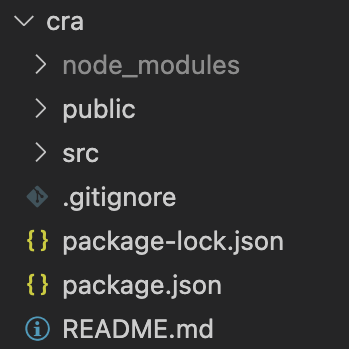
\includegraphics{fileStructureInitCRA}
   \centering
   \caption{Bestandsstructuur nieuw CRA project}
\end{figure}

Alles wat in de public map staat, zijn statische assets. Deze zullen via een url bereikbaar zijn. Als we kijken in het index.html bestand, merken we op dat er geen enkele script-tag aanwezig is. Hierover later meer.
In de src map staat alles wat door Webpack zal gebundeld worden. Standaard worden er CSS bestanden aangemaakt voor styling en een logo in svg formaat. Dit wordt gedaan om aan te tonen dat we deze assets gewoon in de Javascript code kunnen importeren, de bundler kan hiermee overweg.

\lstinputlisting[language=Javascript]{codeSnippets/importCSS.js}

In het package.json bestand staat er allemaal info over dit project. In het dependencies gedeelte staan alle externe packages die dit project gebruikt. Nieuwe packages worden gedownload aan de hand van Node Package Manager of NPM. Bij de dependencies staat een package genaamd “react-scripts”.
React-scripts \autocite{facebook-2018} is een package gemaakt door de makers van React en is de motor achter CRA.
Wat voor dit onderzoek relevant is, is dat het de Webpack.config bevat. Dit bestand bestaat uit maar liefst 700+ lijnen code \autocite{facebook-2021}. Nu is de reden dat we CRA gebruiken en niet van nul beginnen, duidelijk.

De volgende stap is om het project lokaal op te starten. React-scripts gebruikt de ingebouwde ontwikkelingsserver van Webpack. Na het uitvoeren van volgend commando, wordt die server opgestart en opent de webapplicatie in een browser.

\lstinputlisting[language=bash]{codeSnippets/craStart.txt}

\begin{table}[h]
   \centering
   \begin{tabular}{lr}
   \textbf{Grootte project (MB)} & 0,037 \\
   \textbf{Grootte node\_modules (MB)} & 214,1 \\
   \textbf{Grootte uitvoer (MB)} & 0,514 \\
   \textbf{Snelheid creatie uitvoer (s)} & 3,67 \\
   \textbf{} & 5 \\
   \textbf{} & 3 \\
   \textbf{} & 3 \\
   \textbf{Snelheid opstarten ontwikkelings server (s)} & 2,67 \\
   \textbf{} & 4 \\
   \textbf{} & 2 \\
   \textbf{} & 2
   \end{tabular}
   \caption{Overzicht nieuw project met Webpack}
   \end{table}

\section{Parcel}
Bij Webpack gebruikten we een framework om het vele configuratie werk te omzeilen. Bij Parcel is dit niet nodig. Zoals in de literatuurstudie vermeld werkt Parcel op een gelijkaardige manier als Webpack, maar dan met zo min mogelijk configuratie. Om een nieuw project op te zetten, gaan we dus geen framework gebruiken.

Maak een nieuwe map aan waar het project zal leven. Aangezien we van nul beginnen, moeten de bestanden uit figuur 3.2 zelf aangemaakt worden.

\begin{figure}[h]
   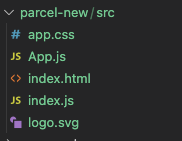
\includegraphics{parcelNew}
       \centering
       \caption{Aan te maken bestanden voor nieuw Parcel project}
   \end{figure}

Hierna moeten er nog enkele packages geïnstalleerd worden, namelijk: React, React-DOM en natuurlijk Parcel. In de package.json moet er ook nog meegegeven worden waar de index.html zich bevindt. Merk op dat er geen apart configuratiebestand voor Parcel is. Nu kan het project opgestart worden met hetzelfde commando als bij Webpack.

 Merk op dat er geen public map aanwezig is zoals in CRA. Er is momenteel geen map waar statische bestanden kunnen leven. Als dit een vereiste is, heeft Parcel een plugin nodig. Gelukkig is die gemakkelijk te installeren.

\section{Snowpack}
Voor Snowpack gaan we net zoals bij Parcel te werk zonder framework. In tegenstelling tot Parcel heeft het Snowpack team al een speciaal react-template gemaakt met een kant en klaar commando om het te initialiseren. Zelf de bestanden aanmaken en dependencies toevoegen is dus niet nodig.

\lstinputlisting[language=bash]{codeSnippets/snowpackNew.txt}
\begin{figure}[h]
   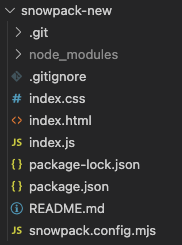
\includegraphics{snowpackNew}
       \centering
       \caption[Aangemaakte bestanden door Snowpack commando]{Aangemaakte bestanden door commado}
   \end{figure}

Deze structuur is identiek aan die van CRA. In tegenstelling tot Parcel is een public map al geconfigureerd voor statische bestanden, zoals afbeeldingen. Een configuratiebestand voor Snowpack is ook aangemaakt. Hierin staan al 25 lijnen configuratie voor ons geschreven. Meer dan Parcel maar aanzienlijk minder dan CRA. Merk op dat sommige bestanden nu de extensie .jsx in plaats van .js hebben. Dit komt doordat Snowpack geen JSX tolereert in .js bestanden. JSX is wat een React component retourneert i.e elk React component moet een .jsx extensie hebben. Geen probleem bij een nieuw project maar bij een oud kan het nodig zijn om vele bestanden van extensie te veranderen, zie later.

Zoals in de literatuurstudie vermeld, is Snowpack geen module bundler aangezien het de verschillende bestanden in een project niet bundelt. In productie kan dat optioneel nog gedaan worden door Webpack of Rollup maar dat is niet standaard. In ontwikkelings heeft dit het grote voordeel dat de bundel niet telkens opnieuw opgebouwd moet worden als een bestand veranderd.

\section{Vite}
Vite is nog een voorbeeld van een ongebundelde build tool, net zoals Snowpack. Een nieuw project opzetten is heel gemakkelijk aan de hand van een simpel commando dat ze voorzien hebben, net zoals Snowpack.

\lstinputlisting[language=bash]{codeSnippets/viteNew.txt}

\begin{figure}[h]
   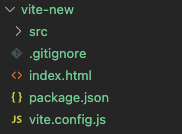
\includegraphics{viteNew}
       \centering
       \caption[Aangemaakte bestanden door Vite commando]{Aangemaakte bestanden door commado}
   \end{figure}

Er is een klein config bestand aanwezig van 7 lijnen code waar de react plugin is geïnitialiseerd. Voor de rest ziet het project in grote lijnen er uit als dat van Snowpack. Er is geen public map aanwezig maar dat kan aangemaakt worden en wordt automatisch geconfigureerd.


\section{Conclusie}
Al de build tools hebben niet gezweet bij het opzetten van een nieuw project, wat maar normaal is. Voor Webpack is er gebruik gemaakt van een framework, CRA, omdat het configuratie werk anders te veel zou zijn. Ook al is het een nieuw project en dus relatief klein, toch kunnen we al verschillen waarnemen tussen de vier kandidaten.

Op onderstaande figuur zien we al een trend verschijnen die doorheen deze conclusie zal gelden: Webpack is aanzienlijk trager dan de competitie, ondanks dat Snowpack niet bundelt, is het toch even traag of trager dan Parcel. Die laatste zijn Rust compiler, zie literatuurstudie, zal zijn vruchten afwerpen. De drie balkjes die ontbreken bij Vite en het ene bij Parcel zijn geen fout: zij waren gewoon sneller dan een volledige seconde.

\begin{figure}[h]
   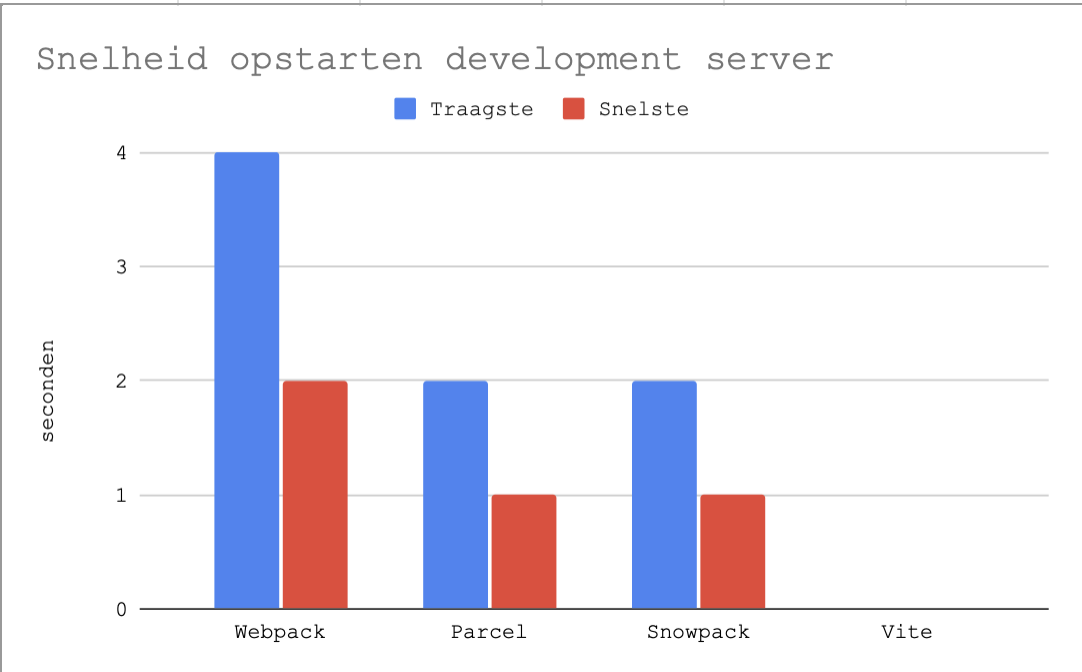
\includegraphics[scale=0.6]{conslusieNieuwDev}
       \centering
       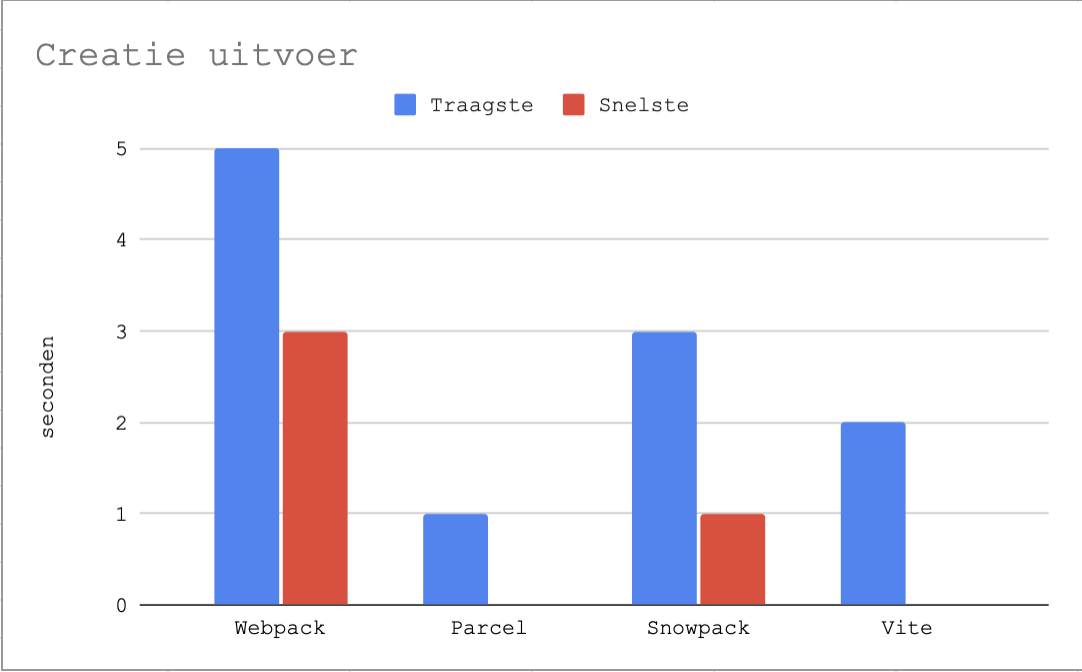
\includegraphics[scale=0.6]{conclusieNieuwUitvoer}
       \centering
       \caption{Resultaten nieuw project}
   \end{figure}


De developer experience was voor al de build tools zo goed als dezelfde bij het opzetten van dit nieuw project. De conclusie kunnen we daarop dus niet baseren. Maar de data hierboven is duidelijk genoeg: bij het opzetten van een project is Vite de beste optie. Het gebruikt het beste van beide werelden: ongebundelde code in ontwikkeling en gebundelde code in productie. De andere opties hebben niet direct een afknapper, maar de snelheid van Vite valt niet te negeren.

\chapter{Bestaand project}

In het vorig hoofdstuk, werden nieuwe projecten opgezet met de respectievelijke build tools. In dit hoofdstuk worden bestaande projecten, opgezet met Webpack, omgevormd zodat ze gebruik maken van de andere opties. Per project wordt eerst wat toelichting gegeven en vervolgens per build tool wat er nodig is om ze werkende te krijgen.

Er is dus nood aan bestaande projecten om de build tools te kunnen testen. Gelukkig zijn er online genoeg open-source voorbeelden hiervan te vinden. Drie projecten werden gekozen aan de hand van hun grootte en technologieën die ze gebruiken. Eén eigenschap hebben ze allemaal gemeen: het zijn Javascript projecten die React als UI library gebruiken. De reden dat geen projecten gekozen werden met andere UI libraries zoals Vue, is omdat React veel meer gebruikt wordt, ook door de co-promotor. Desondanks zijn de gekozen projecten ook representatief voor de andere UI libraries aangezien ze uiteindelijk allemaal Javascript zijn.

\section{Mortage}
Het eerste project dat we gaan omvormen is de Mortage Overpayment Calculator \autocite{houghton-2019}.
Het is een zeer simpel en klein project van 17 KB groot dat is opgezet met CRA.
Daarnaast maakt het nog gebruik van andere open-source packages die verzameld worden in de nodemodules map.
Die map is 214 MB groot.

Mortage is een ideaal project om mee te starten aangezien het geen speciale technologieën gebruikt. CSS voor stijl, wat de browser begrijpt zonder enige omvorming en voor de rest Javascript en HTML. Normaal zouden we dus niet in de problemen mogen komen. Een potentiële moeilijkheid wat dit project ook vermijdt is een map voor statische bestanden.

\begin{figure}[h]
   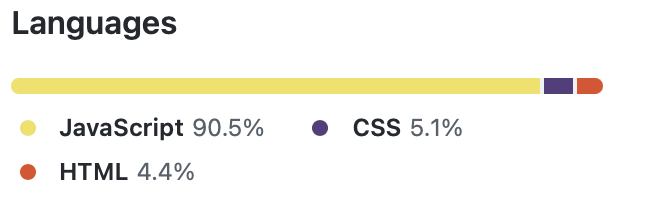
\includegraphics{Mortage_languages}
       \centering
       \caption{Overzicht gebruikte technologieën van het Mortage project}
 \end{figure}

\subsection{Parcel}
Zoals in de literatuurstudie vermeld, probeert Parcel hetzelfde als Webpack te bereiken maar met veel minder tot geen configuratie. Die bewering zal nu nagegaan worden. Mortage is opgezet met CRA en gebruikt dus het react-scripts package die onder andere alle Webpack configuratie op zich neemt. Om Webpack in te ruilen voor Parcel moeten we dus eerst react-scripts bij het grofvuil zetten. Het package.json bestand bevat alle info over een project: de naam, versie, welke andere packages het gebruikt, hoe het wordt opgestart en nog veel meer. Ook Mortage heeft zo’n bestand en dat ziet er als volgt uit:

\lstinputlisting[language=Javascript]{codeSnippets/packageMortage.json}

In het gedeelte “scripts” staan de verschillende commando’s. Het start en build commando starten het project in ontwikkelings- en productiemodus respectievelijk op. Beide voeren op hun beurt een commando van react-scripts uit. Dit gaat dus vervangen moeten worden. In de documentatie van Parcel valt te lezen dat we die commando’s moeten vervangen met de volgende:

\lstinputlisting[language=Javascript]{codeSnippets/scriptsParcelMortage.json}

Vervolgens moet het index.html bestand aangepast worden. Voor de wijzigingen zag het er als volgt uit:

\lstinputlisting[language=HTML]{codeSnippets/mortageIndex.html}

Merk op dat er nergens een verwijzing is naar een Javascript bestand. React-scripts voegt dat automatisch toe bij het bouwen van het project. Parcel doet dat niet dus er moet nog een expliciete verwijzing komen.

\lstinputlisting[language=HTML]{codeSnippets/mortageIndexScript.html}

Nu moet Parcel uiteraard nog gedownload worden. Nadien werkt het project.

\subsection{Snowpack}
Snowpack is een ontwikkelings build tool zoals uitgelegd in de literatuurstudie. Wat dat betekent in de werkelijkheid volgt later. Eerst kijken we hoe Mortage kan omgevormd worden van Webpack naar Snowpack.

Bij Parcel lag de focus op zo weinig mogelijk configuratie, niet bij Snowpack. Snowpack is veel moeilijker te configureren dan Parcel en Vite en voelt in dat opzicht aan als Webpack. We ondernemen dezelfde stappen als hierboven om react-scripts te verwijderen en die te vervangen door de nieuwe commando’s. Daarna voegen we Snowpack toe samen met twee andere plugins voor React. We doen net dezelfde wijzigingen aan index.html, voegen een configuratie bestand toe en proberen de app te runnen. Een foutmelding verschijnt. Om die te kunnen begrijpen, is er eerst wat meer uitleg nodig.

Een React component retourneert JSX. JSX is, zonder te veel in details te gaan, een extensie bovenop Javascript die een manier biedt om de weergave van componenten te structureren en lijkt heel hard op HTML. Het belangrijke om hiervan mee te nemen is dat het een Javascript extensie is. In CRA en sommige andere frameworks is het mogelijk om JSX in een bestand te schrijven met de standaard Javascript extensie .js . Snowpack ondersteunt dit niet. Als een bestand JSX bevat, moet die de extensie .jsx krijgen. Dus moeten we alle bestanden die JSX gebruiken van bestandsextensie veranderen. Hierna werkt de app naar behoren.

\subsubsection{Vite}

Vite combineert het beste van de twee voorgaande build tools. Het is een ontwikkelings build tool in ontwikkelingsmodus en een module bundler in productie, en dat alles zonder al te veel configuratie. Om Mortage op te zetten met Vite overlopen we stappen die eerder al aan bod kwamen: react-scripts verwijderen, index.html voorzien van een script-tag en package.json naar de nieuwe commando’s aanpassen en Vite zelf installeren. Net zoals Snowpack ondersteunt Vite geen JSX in een .js bestand en is er een plugin voor React. In tegenstelling tot Snowpack is de plugin niet nodig om het project werkend te krijgen. Na het aanpassen van de bestandsextensies en eventueel downloaden van de plugin, kan dit project zonder problemen opgestart worden.

\subsection{Todoist}

Todoist \autocite{hadwen-2021} is een simpele to-do webapplicatie. Een gebruiker kan taken toevoegen die nog moeten gedaan worden en aanduiden wanneer die voltooid zijn. Het is een groter project dan Mortage met een grootte van 106KB en 377MB nodemodules maar kan nog steeds beschouwd worden als een kleine tot medium grootte app. Het heeft een database nodig om de taken te kunnen opslaan en zoals hieronder te zien is, gebruikt het een andere taal voor stijl: SCSS. SCSS is een superset of uitbreiding van gewone CSS. Aangezien een webbrowser die uitbreiding niet ondersteunt, moet het SCSS bestand omgevormd worden naar gewone CSS wanneer de applicatie start. Dit kan eventueel tot extra configuratie leiden bij het instellen van een nieuwe build tool.

\begin{figure}[h]
   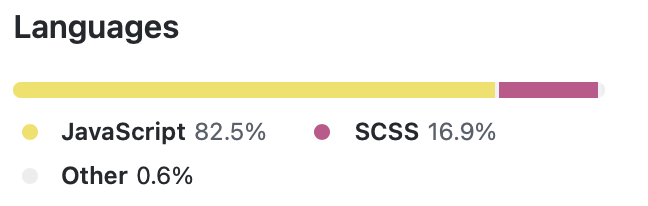
\includegraphics{Todoist_languages}
       \centering
       \caption{Overzicht gebruikte technologieën van het Todoist project}
   \end{figure}

\subsubsection{Parcel}

Om dit project om te vormen naar Parcel worden eerst dezelfde stappen overlopen als in het vorige Parcel project. Er zijn twee mogelijke extra struikelblokken bij Todoist: het gebruik van SCSS en statische bestanden. Het eerste overkomt Parcel met glans: we moeten niets zelf configureren. De eerste keer dat Todoist wordt gestart, detecteert Parcel dat er SCCS aanwezig is en download de bijhorende plugin. Het tweede probleem vereist ook een plugin en daarenboven nog wat configuratie. In de package.json duiden we met enkele lijnen aan waar het mapje met statische bestanden zich bevindt. Nadien moeten de verwijzingen naar de afbeeldingen nog veranderd worden naar de nieuwe locatie. Hierna is ook dit project bijna klaar voor gebruik. Enkel nog het configuratie bestand voor de database moet nog aangepast worden.

\subsubsection{Snowpack}

Ook hier zijn de stappen gelijkaardig aan het vorig project. Na die te doorlopen volgen de twee potentiële moeilijkheden. In het vorig deel over Snowpack werd al vermeld dat statistische bestanden ondersteund worden zonder extra plugin. Het tweede probleem, SCSS, kan eveneens opgelost worden door een plugin. In tegenstelling tot Parcel, moet die wel manueel toegevoegd worden.

\subsubsection{Vite}

Voor Vite kunnen we heel kort blijven. Na het uitvoeren van dezelfde stappen als vorig project, werkt alles. Zowel statische bestanden als SCCS zijn ondersteunt zonder extra plugins of configuratie.

\subsection{Bar}
Als laatste nemen we het grootste en meest complexe project van deze studie onder de loep. De BarApp \autocite{vansteenkiste-2021} is ontworpen om barlijsten bij te houden zonder zelf rekening te houden met de effectieve betaling. In vergelijking met de voorgaande projecten is het veel groter: 27MB voor het project zelf en dan nog eens 442MB voor de nodemodules. SCCS valt weg als moeilijkheid en wordt vervangen door twee nieuwe: TypeScript en Tailwind CSS.

\begin{figure}[h]
   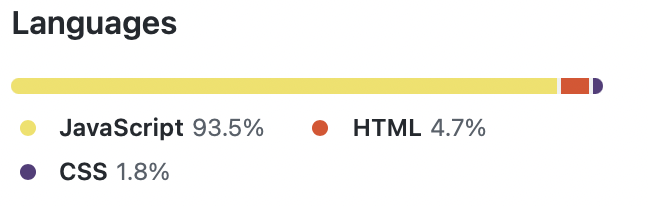
\includegraphics{Barapp_languages}
       \centering
       \caption{Overzicht gebruikte technologieën van het BarApp project}
 \end{figure}

TypeScript is net als SCCS een superset of uitbreiding. Deze keer niet van CSS maar van Javascript. De browser begrijpt geen TypeScript dus moet het eerst vertaald worden naar normale Javascript. De build tools zijn hier verantwoordelijk voor.

De tweede moeilijkheid, Tailwind CSS, staat niet in het gebruikte-talen-overzicht van hierboven. Toch is het iets waar we rekening mee moeten houden. Het is een collectie van allemaal CSS klassen die de gebruiker direct in een JSX element kan gebruiken. Tailwind zelf bevat dus hele grote CSS bestanden om die klassen allemaal te definiëren. Aangezien we enkel de klassen willen behouden die effectief gebruikt worden in het project, worden de ongebruikte gewist bij het bouwen van de applicatie voor productie. Hoewel dit alles geen taak is van de build tool zelf, kunnen er moeilijkheden optreden bij de configuratie.
  
\subsubsection{Parcel}

Nog maar eens overkomt Parcel de mogelijke struikelblokken met zo goed als geen configuratie. Het ondersteunt Typescript zonder iets extra te moeten doen. Naast de standaard configuratie van Tailwind zelf, is er niets anders nodig om het werkend te krijgen. Na het overlopen van de stappen van de vorige Parcel projecten, met in het bijzonder de stap voor statische bestanden, is ook deze applicatie bijna klaar voor gebruik. Voor het laatste detail nemen we nog een kijkje naar de index.html. Aangezien CRA op een andere manier verwijst naar de afbeeldingen die hier staan, moeten de href attributen aangepast worden.

\subsubsection{Snowpack}
Om al een tipje van de sluier op te lichten: dit project was veel lastiger om op te zetten met Snowpack dan met de andere twee opties. Eerst het goede nieuws: Typescript is ook ondersteund zonder extra configuratie. Daar stopt de vreugde al. De overige problemen worden door hun complexiteit in paragrafen onderverdeeld.

Voor Tailwind CSS valt het nog wel mee. Naast dezelfde configuratie en installatie stappen die moeten doorlopen worden als bij Parcel (en Vite), moet er nog een plugin geïnstalleerd worden voor Snowpack zelf. Hierna moet die zijn configuratie bestand aangepast worden zodat de plugin kan werken. Dat doen we door op twee verschillende plaatsen een lijn code toe te voegen.

Zoals in de literatuurstudie uitgelegd, ondersteunen moderne browsers enkel ESM. Aangezien Snowpack een ongebundelde build tool is, stuurt het de bestanden van het project naar de browser zonder ze te bundelen.

\begin{figure}[h]
   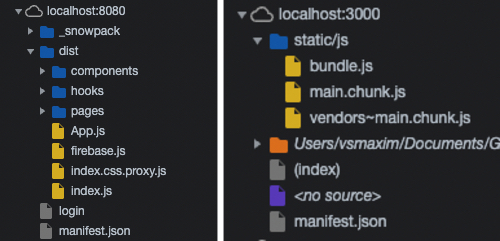
\includegraphics{bundledVSUnbundledFiles}
       \centering
       \caption{Bestandsstructuur ongebundeld vs gebundeld}
 \end{figure}

Merk op dat bij de ongebundelde versie van dit project, de bestandsstructuur dezelfde is als hoe we het project maken. Een bundler zoals Webpack, steekt alle bestanden die naar elkaar verwijzen samen in één bestand dat dan naar de browser gestuurd wordt. ongebundelde build tools zoals Snowpack laten de bestandsstructuur met rust omdat ze vertrouwen op het feit dat moderne browsers ESM ondersteunen. Dus zolang er in het project enkel ESM wordt gebruikt, is er geen probleem. Jammer genoeg staat er in de App.jsx een require functie, een CommonJS module dus. Omdat Snowpack niets doet om dit te vertalen zal de CommonJS module manueel omgevormd moeten worden naar ESM. Gelukkig wordt die vertaling wel uitgevoerd voor de node-modules, want die bevatten ook vaak CommonJS.

Voor het volgend probleem, wordt het index.jsx bestand onder de loep genomen.

\lstinputlisting[language=Javascript]{codeSnippets/indexBar.js}

De aangeduide code vormt een probleem. De lijn process.env.NODE env === “production” wordt gebruikt om te kijken of de app in productie draait of lokaal, in ontwikkelingsmodus. Naast dit voorbeeld wordt deze methode vaak toegepast in dit en andere projecten. Het probleem is dat Snowpack het niet ondersteunt. Omdat dit voorbeeld niet cruciaal is, laten we het weg om Snowpack opgezet te krijgen. Jammer genoeg gebruikt deze app Workbox. Workbox is een Javascript bibliotheek die een PWA opzetten, gemakkelijker maakt. Een PWA is een webapplicatie die installeerbaar is op een Smartphone of computer. Het probleem is dat Workbox ook gebruikt maakt van bovenstaande methode. Als we deze bibliotheek nog steeds zouden willen gebruiken, zou dit alles ook moeten herschreven worden. Voorlopig gaan we verder zonder aangezien het veel tijd in beslag zou nemen. Op naar het laatste probleem.

React kan al even gebruikt worden zonder het te moeten importeren in een bestand. Dat wordt automatisch voor de developer gedaan. Jammer maar helaas: Snowpack ondersteunt dit niet. Aan elk Javascript bestand waar iets van de React methodes gebruikt wordt, moet een import statement toevoegen als volgt:

   \lstinputlisting[language=Javascript]{codeSnippets/importReact.js}

Na dit alles te overlopen, weliswaar zonder PWA-functionaliteit, werkt het project. Eindelijk.

\subsubsection{Vite}
Na de hele waslijst problemen die bij Snowpack opdoken, doet het deugd om weer met Vite aan de slag te mogen gaan. Van de struikelblokken die Snowpack tegenkwam, blijft voor Vite enkel nog het probleem van de CommonJS module over. Na die te herschrijven en dezelfde stappen te doorlopen als bij de vorige Vite secties, werkt dit project volledig, ook Workbox. Typescript is ondersteund zonder extra gedoe en voor Tailwind is de gebruikelijke installatie en configuratie nodig, geen extra plugin. Net zoals bij Parcel moeten de verwijzingen naar de afbeeldingen in de index.html bijgeschaafd worden.

\section{Conclusie}
Een bestaand project omvormen is het heel andere koek gepaard met andere overwegingen. In de methodologie is getracht projecten te kiezen met zoveel mogelijk uiteenlopende technologieën. Natuurlijk is lang niet alles aan bod gekomen. Een project kan bestaan uit talloze combinaties van verschillende, soms niche technologieën, packages of zelf geschreven bibliotheken. Wat in dit onderzoek geconcludeerd zal worden, is een overweging gebaseerd op de projecten die hier aan bod gekomen zijn. Het kan zijn dat voor een ander project, die keuze minder gemakkelijk of zelfs uitgesloten is door welke factor dan ook. Dat terzijde, de conclusie zal in het algemeen voor de meeste gelden aangezien veel voorkomende use-cases aan bod kwamen. Onderstaande resultaten zouden hoogstwaarschijnlijk nog kunnen bijgeschaafd worden door van elke build tool de configuratie te optimaliseren per project. Dit echter is niet het punt van deze studie. Welke build tool is in het algemeen de beste keuze, zonder uren de configuratie bij te schaven?

Op onderstaande figuur is te zien dat elke geteste build tool het beter doet dan Webpack en het verschil is vaak niet klein. Hoewel Snowpack ook aanzienlijk sneller is maar uit de methodologie bleek is dat de developer experience ver van optimaal is, zeker in vergelijking met de andere opties, kijk je beter elders bij het kiezen van een nieuwe build tool. Parcel en Vite daarentegen doen het heel goed op vlak van developer experience en snelheid. Parcel levert gebundelde code af, ook in ontwikkelingsmodus. Dit kan een voor- of nadeel zijn, afhangend hoe het bekeken wordt. Uit het vorig hoofdstuk blijkt dat Vite geen CommonJS ondersteunt, Parcel wel. Hoewel Parcel in sommige scenario’s net iets sneller weet te zijn dan Vite, wint die laatste toch in de meeste gevallen. Merk op dat ook bij de tweede grafiek, het balkje bij Vite ontbreekt. Dit is weer geen fout: Vite slaagt erin om zijn ontwikkelingsserver gemiddeld in sneller dan een seconde op te starten. Dat is indrukwekkend, zeker als dit naast de resultaten van de competitie gelegd wordt.

\begin{figure}[h]
   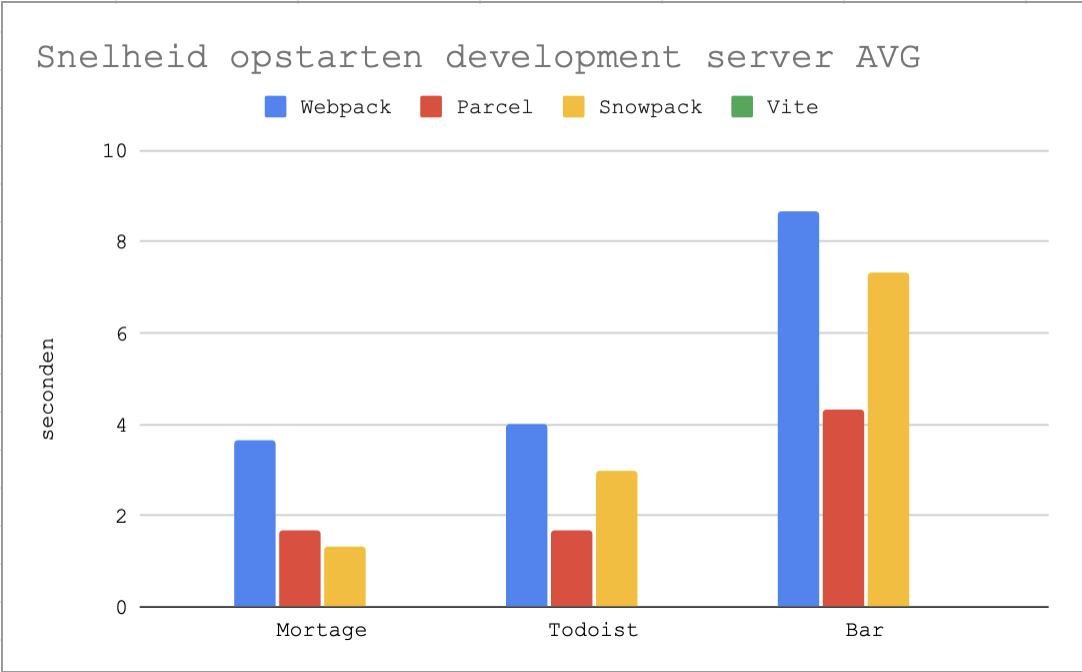
\includegraphics[scale=0.6]{conclusieBestaandDev}
       \centering
       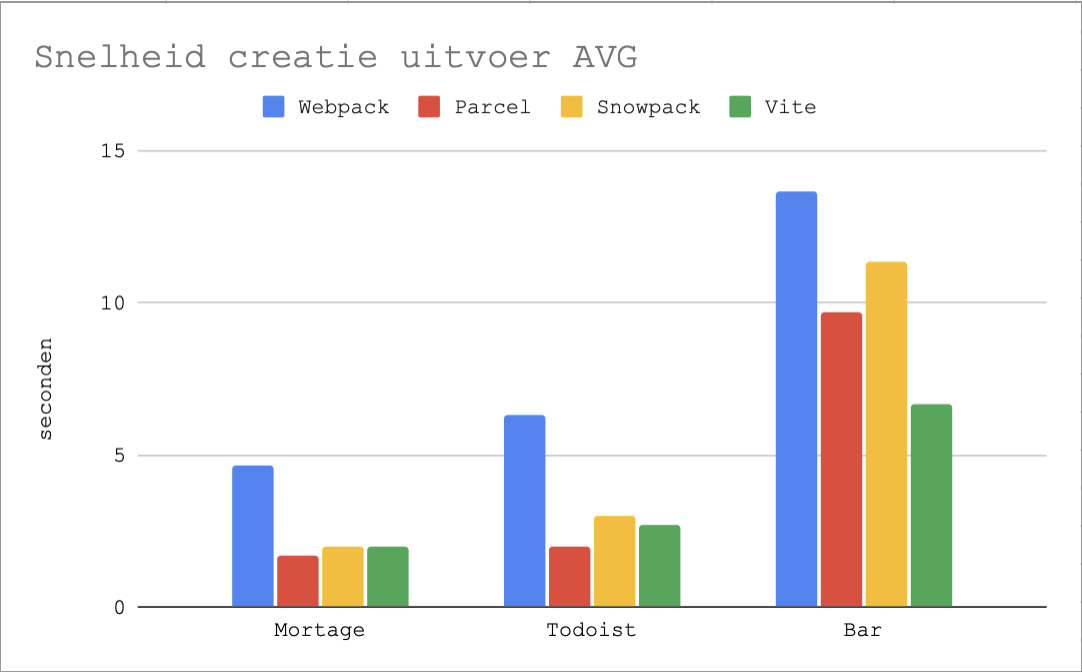
\includegraphics[scale=0.6]{conclusieBestaandUitvoer}
       \centering
       \caption{Resultaten bestaand project}
 \end{figure}
 
